\documentclass[10pt,a4paper]{article}
\usepackage[utf8]{inputenc}
\usepackage{amsmath}
\usepackage{amsfonts}
\usepackage{amssymb}
\usepackage{german}
\usepackage{fancyhdr}
\usepackage{graphicx}
\usepackage{geometry}
\usepackage{color}
\usepackage[usenames,dvipsnames]{xcolor}
\usepackage{DejaVuSans}
\usepackage[T1]{fontenc}
\renewcommand*{\familydefault}{\sfdefault}
\geometry{verbose,a4paper,tmargin=35mm,bmargin=35mm,lmargin=25mm,rmargin=25mm}
\author{Dominik Heeb, Fabian Keller}
\title{Projektplan Semesterarbeit}
\pagestyle{fancy}
\fancyhead{}
\fancyhead[L]{Projektplan - Dynamic Parallel Checker}
\fancyhead[R]{Domink Heeb, Fabian Keller}
\fancyfoot{}
\fancyfoot[R]{Seite \thepage}
\begin{document}
\begin{titlepage}
	\begin{Huge}
		\begin{center}
				Projektplan \\Dynamic Parallel Checker\\[2.0cm]
		\end{center}
	\end{Huge}
	
	\begin{Large}
		\begin{center}
				by Dominik Heeb, Fabian Keller		
		\end{center}
	\end{Large}
\end{titlepage}

\newpage
\tableofcontents 
\newpage

\section{Management Abläufe}
\begin{flushleft}
	Dieses Semesterarbeit wird im Rahmen des Bachelor Studiums an der HSR durchgeführt welches bei erfolgreichem Abschluss mit 8 ECTS Punkten gewertet wird. Ein ECTS Punkt entspricht einem ungefähren Zeitaufwand von 25 bis 30 Stunden. Somit wird von jedem Teammitglied ein Zeitaufwand von ca. 200 bis 250 Stunden erwartet.
\end{flushleft}

\subsection{Zeitliche Planung}
	\begin{flushleft}
		Der zeitliche Projektplan zeigt eine grobe zeitliche Übersicht über die gesamte Semesterarbeit. Über die einzelnen Iterationen und auch Meilensteine.
	\end{flushleft}
	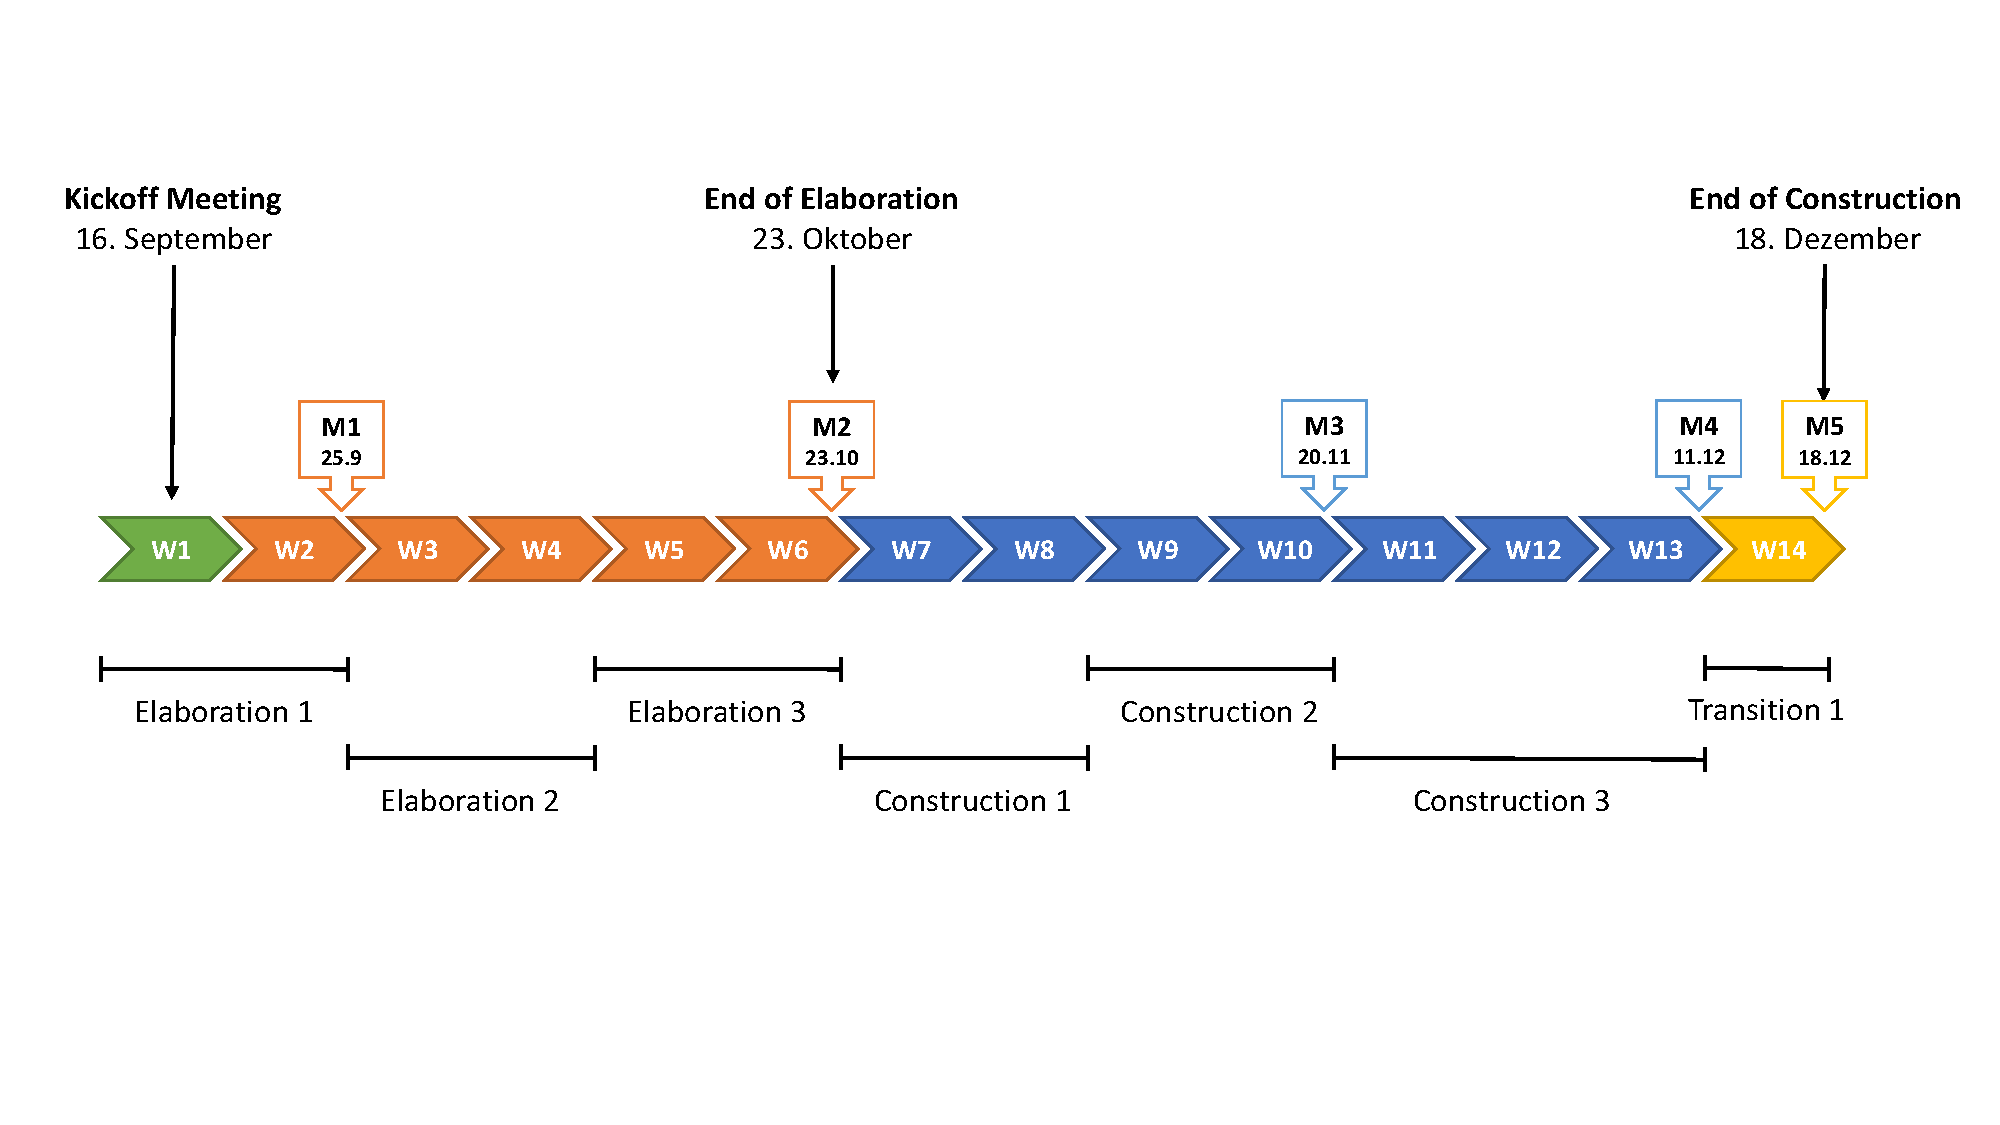
\includegraphics[width=16cm,height=7.5cm,trim=10mm 40mm 0mm 20mm, clip]{pictures/Meilensteinplan.pdf}

\subsection{Meilensteine}
\begin{flushleft}
	Die einzelnen Meilensteine, die bereits in der zeitlichen Planung ersichtlich sind, beinhalten folgende Ziele:
\end{flushleft}
\begin{tabular}{cl}
	\textcolor{Orange}{\textbf{M1:}} & Fertigstellung der Projektplanung\\[0.2cm]
	\textcolor{Orange}{\textbf{M2:}} & Auseinandersetzung mit der Thematik, Entscheid welcher Arlgorithmus für Prototyp\\[0.2cm]
	\textcolor{NavyBlue}{\textbf{M3:}} & Race Conditions werden mit Hilfe des Prototyp erkannt\\[0.2cm]
	\textcolor{NavyBlue}{\textbf{M4:}} & Prototyp ist fertig implementiert und integriert.\\[0.2cm]
	\textcolor{Dandelion}{\textbf{M5:}} & Abschluss des Projekts, Abgabe der technischen Dokumentation, Poster und Kurzfassung\\
\end{tabular}
\subsection{Besprechungen}
\begin{flushleft}
	Die Besprechung findet jede Woche am Dienstag im IFS (Institute for Software) Raum 6.108 um 14:00 Uhr statt. In dieser Besprechung wird der aktuelle Status der Semesterarbeit überprüft und offene Fragen geklärt.\\
	Vor jeder Besprechung sendet das Projektteam dem Betreuer eine Liste der zu behandelnden Traktanden und anschliessend ein Protokoll der Besprechung.
\end{flushleft}
\newpage
\section{Vorgehen}
\subsection{Projektmanagement}
\subsubsection{Aufbau}
Das Projekt wird gemäss RUP durchgeführt.\\
Die Phasen sind folgendermassen aufgeteilt\\
\begin{itemize}
	\item Elaboration: Ziel der Elaboration Phase ist das evaluieren verschiedener Lösungsalgorithmen für ein Dynamic Parallel Checker
	\item Construction: Die Construction Phase wird verwendet, einen funktionsfähigen Parallel Checker Prototyp zu erstellen
	\item Transition: Zusammenstellung des Abschlusspapers und dem Poster
\end{itemize}
\subsubsection{Tools}
Für das Projektmanagement werden folgende Tools verwendet:
\begin{itemize}
\item JIRA: für die Planung und Verwaltung der Arbeitspakete.
\item GitHub: Der Code und die Dokumentation werden über Github Repositories verwaltet
\item CI Server: Mittels eines CI Server wird die Qualität und Lauffähigkeit des Codes geprüft
\item Texmaker: Latex Editor für die Dokumentation
\item Visual Studio: IDE für C\#.Net Entwicklung
\end{itemize}
\subsection{Entwicklung}
\subsubsection{Vorgehen}
Die Entwicklung des Parallel Checkers wird als Agiles Softwareprojekt aufgebaut.
\subsubsection{Unit Testing}
Die Entwicklung des Dynamic Parallel Checkers wird mittels Unit Tests auf seine Qualität geprüft. Diese werden im CI Server laufend durchgeführt und bei Fehlern im Projektmanagementtool JIRA angezeigt
\subsubsection{Code Reviews}
Code Reviews und Pair Programming sind Methoden um die Qualität des Codes innerhalb des Teams hoch zu halten
\subsubsection{Code Analyse}
Um einen einheitlichen Code zu gewährleisten wird Resharper auf den Entwicklungsumgebungen, so wie dem CI Server installiert
\subsubsection{Code Style Guidelines}
Der C\# Code wird gemäss den Microsoft Coding Guidlines entwickelt.
\end{document}